

\title{\papertitle}
\author{Rocco Schulz, Max V\"{o}kler, Joe Boden,\\ Robert Wawrzyniak, Can Paul Bineytioglu\\\\
	Corporate State University\\Baden-Wuerttemberg - Stuttgart}

\date{\today}

\begin{document}

\maketitle

\begin{abstract}
This paper evaluates asynchronous server technologies. Strenghts and weaknesses
of asynchronous programming models are elaborated and a proof of concept 
based on node.js and vert.x is used to evaluate non-functional attributes such as
maintainability. \ldots
\end{abstract}
\newpage

\tableofcontents
\newpage

\listoffigures
\addcontentsline{toc}{section}{List of Figures}
\newpage

\printnomenclature
\addcontentsline{toc}{section}{\nomname}
\newpage

\section{Introduction}

In traditional web application development data is transmitted synchronously, i.e. upon a GET/POST request the result can be displayed only after transmission and processing are finished, as highlighted in figure \ref{img_req_res}\footcite{req_res}. While maintaining simplicity and predictability this can cause serious latency when uploading large pieces of data most commonly complex forms for registration. Naturally rich content such as images and videos causes even more waiting.

\begin{figure}[hbtp]
\centering
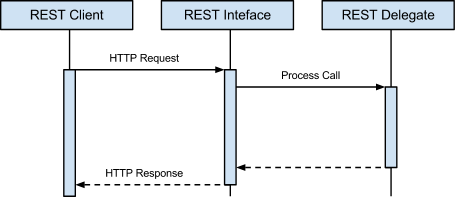
\includegraphics[scale=0.75]{img/image01.png}
\caption{REST request-response sequence diagram\label{img_req_res}}
\end{figure}

As demands around collaborative access and media richness evolved, this became a serious bottleneck, essentially preventing these types of applications. On the client-, i.e. browser-, side developers were able to work around the issue of synchronous transmission using the XmlHttpRequest object which allows to request resources programmatically (using JS\nomenclature{JS}{JavaScript}) while deferring handling of the response to a callback (see figure \ref{img_ajax}\footcite{img_ajax}) thus enabling much more responsive software.

\begin{figure}[hbtp]
\centering
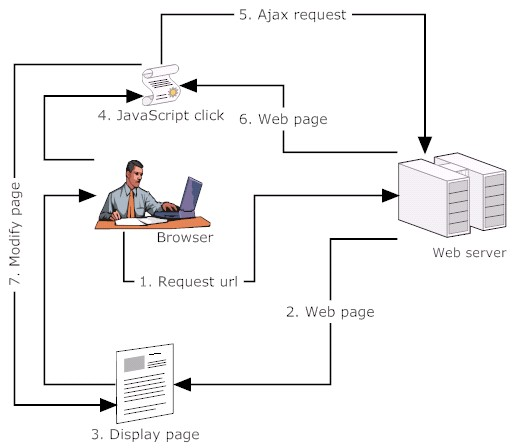
\includegraphics[scale=0.5]{img/ajax-diagram}
\caption{AJAX Diagram\label{img_ajax}}
\end{figure}

Although this addressed the issue on the client-side, server-side request were still handled very much in a synchronous fashion. For example the popular Apache web server forks a new process for each incoming request\footnote{TODO: find source}. As popular applications have to cope with unprecedented amounts of concurrent users in conjunctions with massive request counts, this obviously causes performance issues.\\

Relatively young frameworks such as Node.js and Vert.x try to address this issue 
by providing a completely asynchronous programming model which allows associating
multiple simultanious connections with a single thread by using an event-driven approach.

%Goal of this paper and structure
This paper elaborates the concepts behind these young frameworks and analyses their 
technical strengths and weaknesses. Furthermore non-functional attributes will be
evaluated based on two sample implementations in Node.js  and Vert.x.

\section{Setting the context}
\label{setting_the_context}

\subsection{Comparison between Asynchronous and Synchronous Processing}
\label{comparison}

%Synchronous calls -> idling threads -> 
A common case in programming is access to I/O.
In synchronous processing a running thread needs to wait for the completion of
the I/O operation before it can continue.
The thread is in an idle state while it is waiting which allows another process 
or thread to occupy the CPU in the meanwhile.\\

% writing multithreaded code is not trivial
In multithreaded applications several threads can run simultaniously within one 
process. Several threads can access shared memory concurrently which can
cause inconcistent states. This can be avoided by synchronizing threads - e.g.
with locks. This means that programmers need to take into account every possible
execution order to effectively avoid program defects such as data races and 
deadlocks.\footcite[Cf.][10]{Breshears_2009}
This can be time consuming and potentially results in error-prone code.

A typical synchronous call is provided in listing \ref{lst:synchronous_call}. The
contents of a file are read and displayed afterwards. The programm is blocked until the
read operation has finished.

% reading a file and displaying it, pseudo code
\lstinputlisting[language=JavaScript,caption={Pseudocode: Synchronously reading and displaying a file's contents},
label=lst:synchronous_call]{lst/synchronous_call.txt}


Asynchronous programming style uses a different concept. The flow of an
application is determined by events, which is why this style is also called
event-driven programming.\footcite[Cf.][16]{teixeira_2012} In listing \ref{lst:asynchronous_call} the call
to the \textit{readAsText} function is done asynchronously. There is no
return value - instead an event handler is provided as a second argument.
This function is also referred to as a callback function. It is called
as soon as the read operation has completed.

% same example as above but with callbacks / events
\lstinputlisting[language=JavaScript,caption={Pseudocode: Asynchronously reading and displaying a file's contents},
label=lst:asynchronous_call]{lst/asynchronous_call.txt}

This concept is coupled with an event loop, which is a single thread that is
running inside the main process.
The loop constantly checks for new events. When an event is detected, the loop
invokes the corresponding callback function. The callback is processed in the
same thread which means that there is at most one callback running at a time.
The event loop continues when the callback has completed. As a result the
developer does not need to take care of concurrency issues during development.
But the developer's task is to write light event handlers that can be processed
quickly as every callback is an interruption of the event processing in the
event loop. \footcite[Cf.][]{Croucher_2010} Memory or processor intense callbacks
can lead to growing queues of unserved events which eventuelly results
in a slow application or service\footcite[Cf.][48]{teixeira_2012}.


% implication: 
% all code should be as non-blocking and asynchronous as possible
% using blocking APIs inside the asynchronous code can cause blocking of the event loop
% which is evil. This is why node.js is based on javacript. Other languages already have
% lots of modules with blocking APIs which could confuse dumb developers.



\subsection{Existing Asynchronous Frameworks}
\label{existing_frameworks}


\subsubsection{Overview}
\label{frameworks_overview}

\FloatBarrier

\begin{savenotes} %alloows proper citation marks inside tables
\begin{table}[h]
\centering
\begin{tabular*}{\textwidth}{p{0.2\textwidth} p{0.15\textwidth} p{0.57\textwidth}}
\toprule
\textbf{Name} & \textbf{Language/s} & \textbf{Description} \\
\midrule 
Twisted			& Python			& ``Twisted is an event-driven networking engine written in 
									  Python and licensed under the open source MIT license"\footcite[Cf.][]{Twisted_2012}.
									  Twisted is a mature framework with a large number of supported networking
									  protocols. Its development is backed by an active
									  community.\footcite[Cf.][12]{fettig_2005}
									  \\
									  
EventMachine 	& Ruby    			& ``EventMachine is a library for Ruby, C++, and Java
									  programs. It provides event-driven I/O using the Reactor 
									  pattern."\footcite[][]{eventmachine_2012}\\

Node.js			& JavaScript		& Node is based on Chrome's JavaScript runtime \textit{V8}.
									  The platform is fully event-driven and offers core
									  functionalities for network programming. Its functionality
									  can be extended with a large number of modules using an
									  integrated package management system.
									  Node.js started development in 2009 and the community
									  is growing since that.\footcite[Cf.][]{Mashtable_2011}\\
									  
Vert.x			& JavaScript, Java, Python, Groovy, Ruby, Coffeescript		
									& A JVM based platform for network applications which is
									  inspired by Node.js. Vert.x comes with its own event
									  bus system that allows distributing applications
									  among multiple network nodes. Support for the languages
									  Scala and Clojure is scheduled for future releases.\footcite[Cf.][]{vertx_2012}\\
\bottomrule 
\end{tabular*}
  \captionof{table}{Existing asynchronous programming frameworks}
  \label{tab:existing_frameworks}
\end{table}
\end{savenotes}


\FloatBarrier

\subsubsection{Node.js}
\label{node.js}

To put it in a nutshell one can say, that Node.js is JavaScript on a server.\\
Besides, Node.js is a young platform with a lot of buzz around it. Due to the
rising of the Web 2.0 and widely accessible internet through smartphones,
demanding users expect more complex and more interactive forms of application usage. 
The challenge even gets harder considering the steep number of
devices that are interacting with online services.%TODO: reference?
To overcome those problems Node.js lays it's foundations on an event driven
computing architecture for web servers.\\
% The paradigm of the event driven programming style is easily explained using a
% real world example. What would you do if you are slicing onions while the turkey
% is nearly on fire in the stove? Right, finishing the slice, turning down the
% heat and opening the oven before getting back to slice some onion rings would be
% a reasonable behavior. The truth is, that browser based programming isn't that
% real life oriented. A lot of techniques try to make real-time and parallelism
% work. Which means continuing slicing during you try to safe the turkey.
Node.js doesn't try to make you perform undoable things. It rather lets events drive the
action, so that it is single-threaded and only one thing happens at once. This
is why an event loop is a fundamental part of Node.js. It includes the concept
of nonblocking I/O activities. A result is that actions that cause the program
to wait like database requests and file I/O  do not halt execution until they
return data. In contrast they process independently and raise an event when the
data is accessible. It is therefore necessary to use callbacks for dealing with
different kinds of I/O.\\
An exemplary code for a basic HTTP server in Node.js is shown in listing
\ref{lst:simple_server} to deepen the understandin gof the event loop and
callback in Node.js.

% reading a file and displaying it
\lstinputlisting[language=JavaScript,caption={The simplest way to programm a server in Node.js},
label=lst:simple_server]{lst/simple_server.txt}



The code uses a factory method to create a new HTTP server and attaches the
argument of the createServer function as a callback to the request event. The
first run of this code is also called setup. When a HTTP request arrives the
anonymous callback function is processed and "Hello World" appears on the
browser.\\
That the basic code above isn't the most sophisticated way to write Node.js code
explains the following thought experiment: Assuming that the Hello World page
would be popular and had a lot of requests from different devices to handle and
in addition the callback processing would take one second, it is obvious that the second
request would already have to wait for one second until it gets served. This is far away 
from the near-real-time requirement Node.js is confronted with.\\
Two programming rules in Node.js can be inferred from the basic server and it's
event loop blocking problem, which is described in section \ref{setting_the_context}.
First, once the setup is in place all actions should be programmed event-driven.
Second, if a workload requires Node.js to process something for a long time,
it should be outsourced to web workers.\footcite[Cf.][]{Croucher_2012}



\subsubsection{Vert.x}
\label{vert.x}

Vertx is a polyglot that runs on the JVM (Java Virtual Machine). It is hence
possible to scale over available cores without manually forking multiple
servers.\\
The application API is exposed in multiple programming lanugages (see table
\ref{tab:existing_frameworks}).
% Implication: use case, code reuse from different legacy systems written in
% different languages

In Vert.x the smallest available deployment unit is a verticle, which runs
inside an instance. Each instance runs singlethreaded.
Multiple verticles can be run inside one instance as depicted in figure
\ref{fig:vertx_constructs}.
%http://vertx.io/core_manual_java.html scaling tcp servers

\begin{figure}[h]
	\centering
	\setlength\fboxsep{2pt}
	\fbox{
	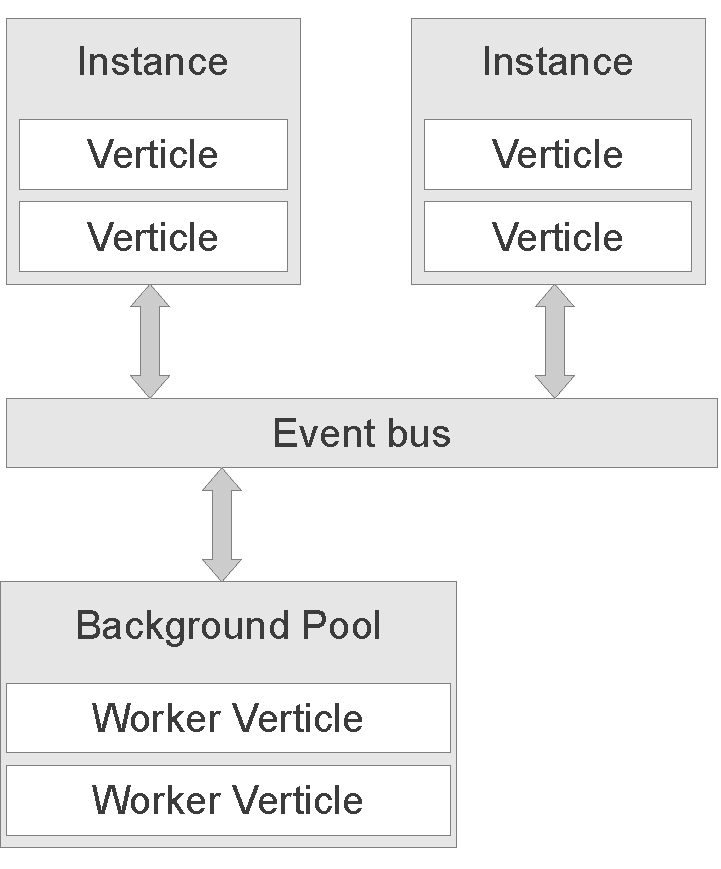
\includegraphics[width=0.4\textwidth]{img/vertx_constructs.pdf}
	}
	\caption{Abstracted deployment units of Vert.x}
	\label{fig:vertx_constructs}
\end{figure}

When multiple instances are run on one machine, Vert.x automatically distributes incoming
requests among all running instances in a round-robin fashion, so that each
vert.x verticle instance remains single threaded.

Vert.x also includes a distributed event bus, which enables verticles to
communicate with each other, either within the same instance or across different
instances. The event bus allows direct communication with in-browser JavaScript as well.\\
% Implication: ideal for real time applications. easy communication between client and server using JS
Vert.x allows to run IO heavy tasks in separate worker threads that reside in a
so-called background pool as these tasks would otherwise block the event loop as
described in section \ref{comparison}.

The core functionality of Vert.x covers basic networking tasks and protocols,
web servers, clients, access to the file system, shared maps and the event bus.
The core libraries of Vert.x can be embedded in any JVM program for reuse in
larger projects.\\
As opposed to Node.js, the core functionality and API can be considered quite
static as changes need to be done in all supported
languages.\footcite[Cf.][]{vertx_2012}\\ % The core can be extended with
The core can be exctended with additional features that are provided by optional
modules that can be obtained over a public git-based module
repository.\footcite[Cf.][]{vertx_mod_2012}.
The repository currently contains 16 distinct modules in different
versions.\footcite[Cf.][]{Vertx_repository_2012}

An extensive online documentation is available for all supported languages.
Additionally, code examples for most features are available for all supported languages in
a public repository\footcite[Cf.][]{Fox_2013}.\\
Vert.x is open source and licensed under the Apache Software License
2.0\footnote{See \url{http://www.apache.org/licenses/LICENSE-2.0.html}}, so that
commecial redistribution in closed source projects should not be an issue.





\section{Areas of Application}
\label{areas_of_application}

\subsection{Use Cases}
\label{use_cases}
The non-blocking nature of asynchronous calls is important in all types of
applications that need to handle a large number of requests in real time.\\
Some success stories are available on \url{http://nodejs.org/}.

Could be used for: 
\begin{itemize}
  \item networked applications that tend to keep many inactive connections
  \item web trackers
  \item web servers
  \item lightweight json APIs (non-blocking I/O model 
  		combined with JavaScript make it a great choice for
  		wrapping other data sources such as databases or web 
  		services and exposing them via a JSON interface)%see http://nodeguide.com/convincing_the_boss.htm
  \item proxies
  \item email and messaging systems
  \item authorization processors
  \item Streaming data (e.g. file uploads in real time)
\end{itemize}

\subsection{Don't use cases and anticipated issues}
\label{dont_use_cases}


As with all technologies one has to carefully decide whether or not it suits the requirements
of a project.


\begin{itemize}
  \item Systems that do a lot of computing / IO access
  \item Datawarehousing with analytics / analytical tasks on large filesets
  \item CRUD / HTML applications*: At present node and vertx do not provide additional
  		benefits to acalability for these types of web applications.
  		Powerfull frameworks like Ruby On Rails,
  		Grails and Django are currently better suited. Providing an app that is suited for 
  		millions of requests does not automatically increase the number of requests.
  \item Desktop applications*: Some frameworks are suited for this, but not node.js.
  		JavaScript is missing operators for good OS integration.
\end{itemize}

Anticipated issues\\

\begin{itemize}
  \item running worker threads does introduce the concurrency issues that were
  		avoided with the event loop again as they could concurrently access IO
  \item \ldots
\end{itemize}
    

    



\section{Exemplary Implementations}
\label{exemplary_implementations}

A simple web form application has been implemented in Node.js and Vert.x to
further analyze non-functional requirements and collect practical experience
with these frameworks.

\subsection{Software Description}
\label{software_description}
Brief description of the insurance fee calculator

\subsection{Software Design}
\label{software_design}
High level design\\
Interface description, and differences between Node.js and Vert.x

\subsection{Software Implementation}
\label{software_implementation}
Complications or any other notes on the implementation process that might be of
importance for the evaluation.





\section{Evaluation of Non-functional Attributes}
\label{evaluation_nonfunctional}

\subsection{Maintainability}
\label{maintainability}
Language: JavaScript is wide spread, same for Java. However JavaScript offers
better flexibility and native constructs for these types of applications.
(Java 8 might improve things a bit).
Node's API is undergoing backwards incompatible changes from time to time.
It is desired to updated some components of a Node based application from
time to time.

\subsection{Integration}
\label{integration}
Vert.x and Node.js are supposed to be used as fully event driven standalone
applications that can be extended with event-driven modules.
However it might be desired to reuse existing software that is not fully event
driven.
Dont make use of blocking apis.
Consider connecting that software with a message bus.
Separate IO intense tasks into ``web workers'' or similar constructs.

\subsection{Scalability}
\label{scalability}
Support for single machine scaling using multiple threads exists.
Deployment on distributed systems differs in node.js and vert.x.
Vert.x. uses its own communication bus to share information between verticles.


\section{Conclusion}
\label{conclusion}
